\documentclass[../Funzionalita.tex]{subfiles}

\begin{document}
\subsection{Area sviluppatore}
\label{subsec:AreaSviluppatore}
	
	\subsubsection{Panoramica}
		Selezionata dal menu dell'applicazione, l'opzione \textit{Area sviluppatore} offre la possibilità di raccogliere e salvare un file Log che contiene tutti i dati dei beacon rilevati finché il Log non è arrestato.
		
		\MainDeveloperPresenter\ è la classe che si occupa di controllare l'accesso a tale area:
		\begin{itemize}
			\item se l'utente ha già inserito correttamente almeno una volta la password gli viene mostrata la lista dei Log salvati;
			\item se l'utente non ha mai inserito correttamente gli viene chiesto il codice sviluppatore.
		\end{itemize}
		
		\MainDeveloperActivity\ invece si occupa della gestione delle opzioni sviluppatore:
		\begin{itemize}
			\item visualizzazione lista log salvati localmente nel device;
			\item passare alla visualizzazione dettagliata log;
			\item avviare un nuovo log.
		\end{itemize}
			

	\subsubsection{Interfaccia grafica}
		L'area sviluppatore è composta da diverse viste. Selezionando dal menu \textit{Area sviluppatore} si vede la vista descritta in \DeveloperUnlockerView\ la quale richiede l'inserimento di una password. Una volta effettuato correttamente l'accesso viene mostrata \MainDeveloperView\ dove si presenta una lista dei log salvati e un pulsante per crearne uno nuovo. Alla creazione si passa alla vista \LoggingView. Si può inoltre visualizzare un contenuto di un log per volta selezionandoli in \MainDeveloperView\ e la visualizzazione interna viene gestita da \LogInformationView.
		
			\paragraph*{Componenti interne}
			\begin{itemize}
			
				\item Package:
				\begin{itemize}
					\item[] \view;
				\end{itemize}
				
				\item Interfacce e classi:
				\begin{itemize}
					\item[] \MainDeveloperViewImp, 
					\MainDeveloperView, \DeveloperUnlockerViewImp, \DeveloperUnlockerView, 
					\LoggingViewImp, \LoggingView, 
					\LogInformationViewImp, \LogInformationView;
				\end{itemize}
				
			\end{itemize}
			
			
			\paragraph*{Componenti esterne}
			\begin{itemize}
				\item Interfacce e classi SDK:
				\begin{itemize}
					\item[] \EditText, \Button, \FloatingActionButton, \ListView, \TextView, \Toolbar;
				\end{itemize}
			\end{itemize}
			
			
			Nelle figure \ref{fig:AreaSviluppatore-InserisciPassword} e \ref{fig:AreaSviluppatore-ListaLog_} si indicano i seguenti widget offerti dal kit Android SDK:
			\begin{enumerate}
				\item \EditText;
				\item \Button;
				\item \Toolbar;
				\item \ListView;
				\item \FloatingActionButton;
			\end{enumerate}
			
			\begin{figure} [h]
				\centering
				
				\subfloat[][Area sviluppatore - Inserimento password]
				{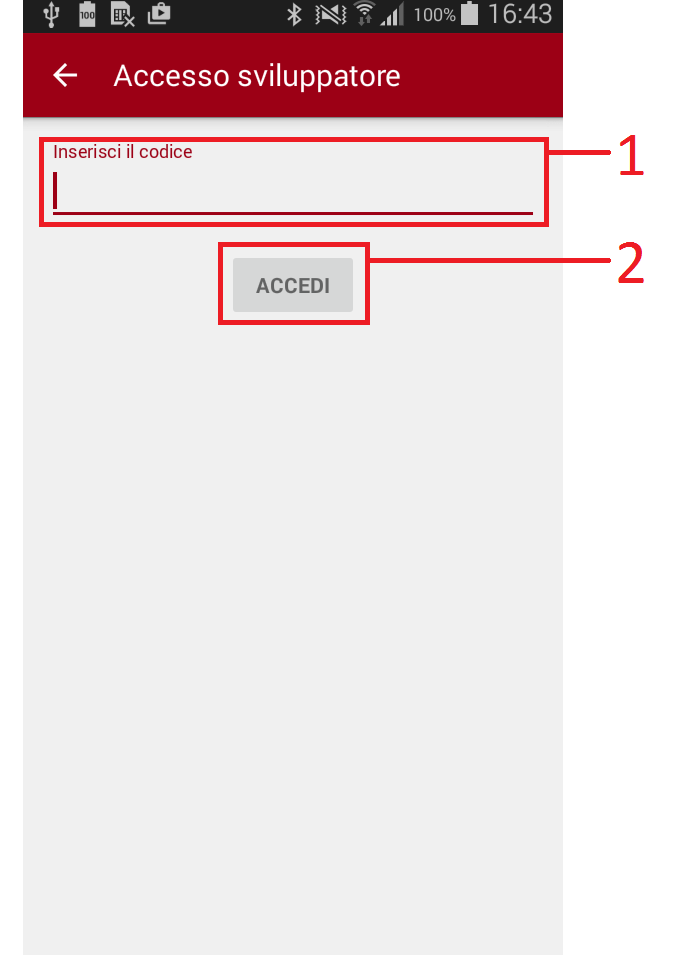
\includegraphics[width=0.3\textwidth]{img/AreaSviluppatore-InserisciPassword_}
				\label{fig:AreaSviluppatore-InserisciPassword}} \quad
				\hspace{1.5cm}
				\subfloat[][Area sviluppatore - Visualizzazione lista log salvati]
				{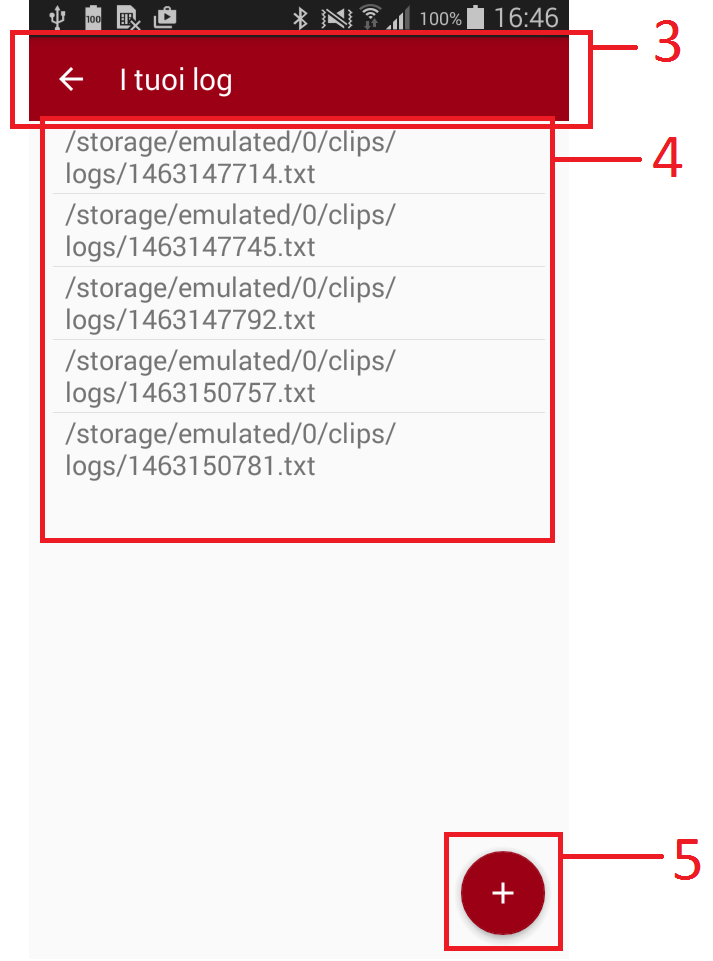
\includegraphics[width=0.3\textwidth]{img/AreaSviluppatore-ListaLog_}
				\label{fig:AreaSviluppatore-ListaLog_}} \\
				\caption{Area sviluppatore}
			\end{figure}
			
	\newpage	
	\subsubsection{Presenter}
		Il compito del presenter per questa funzionalità è affidato agli oggetti \MainDeveloperPresenter, \DeveloperUnlockerActivity, \MainDeveloperActivity, \LoggingActivity e \LogInformationActivity.
		\MainDeveloperPresenter\ comunica con \Setting\ per accertarsi se l'utente sia sviluppatore, in tal caso la gestione passa a \MainDeveloperActivity. Nel caso contrario la gestione passa a \DeveloperUnlockerActivity\ la quale richiede la password per accedere all'area sviluppatore. In generale tutte le altre activity comunicano con la classe \InformationManagerImp\ del model e la relazione avviene grazie all'uso della dependency injection.
	
		\paragraph*{Componenti interne}
			\begin{itemize}
			
				\item Package:
				\begin{itemize}
					\item[] \view;
					\item[] \presenter;
				\end{itemize}
				
				\item Interfacce e classi:
				\begin{itemize}
					\item[] \MainDeveloperPresenter, \MainDeveloperActivity, \MainDeveloperView, \DeveloperUnlockerActivity, \DeveloperUnlockerView, \LoggingActivity, \LoggingView, \LogInformationActivity, \LogInformationView;
				\end{itemize}
				
			\end{itemize}
			
			
		\paragraph*{Componenti esterne}
			\begin{itemize}
				\item Interfacce e classi SDK:
				\begin{itemize}
					\item[] \AppCompatActivity;
				\end{itemize}
			\end{itemize}
	
	\newpage
	\subsubsection{Logging}
		La classe \InformationManagerImp\ rende disponibile quattro metodi per eseguire l'operazione di logging:
		\begin{itemize}
			\item \lstinline|getLogInfo()| per reperire i riferimenti ai file Log;
			\item \lstinline|startRecordingBeacon()| per far sì che un nuovo file Log sia scritto;
			\item \lstinline|removeBeaconInformationFile()| per rimuovere un file log dal dispositivo;
			\item \lstinline|saveRecordedBeaconInformation()| per salvare il nuovo log inizializzato con \lstinline|startRecordingBeacon()|;
		\end{itemize}
		La classe \Setting\ invece è utilizzata per ottenere il path della cartella in cui sono salvati i Log. Tale path è salvato nelle preferenze dell'applicazione rese disponibili da \SharedPreferences.
		
		\paragraph*{Componenti interne}
			\begin{itemize}
				\item Package:
				\begin{itemize}
					\item[] \model;
					\item[] \usersetting;
				\end{itemize}
				
				\item Interfacce e classi:
				\begin{itemize}
					\item[] \InformationManager, \InformationManagerImp, \Setting;
				\end{itemize}
			\end{itemize}
		
		\paragraph*{Componenti esterne}
			\begin{itemize}
				\item Interfacce e classi SDK:
				\begin{itemize}
					\item[] \SharedPreferences, \Log;
				\end{itemize}
			\end{itemize}

\end{document}
